
\de{ĐỀ THI GIỮA HỌC KỲ II NĂM HỌC 2022-2023}{THPT Gia Định}

\begin{bt}%[Dự án đề kiểm tra GHKII-NH22-23-TinDatTran]%[0T7B2-1]
	Giải bất phương trình $ 5x^2-4x-1 \leq 0$.
	\loigiai{
	Cho $ 5x^2-4x-1 =0 \Leftrightarrow \hoac{&x=-\dfrac{1}{5}\\&x=1.}$\\
	Bảng xét dấu
	\begin{center}
		\begin{tikzpicture}
\tkzTabInit[nocadre=false,lgt=3,espcl=2.5,deltacl=0.6]
		{$x$/1, $5x^2-4x-1$ /0.6}
		{$-\infty$,$-\dfrac{1}{5}$,$1$,$+\infty$}
		\tkzTabLine{,+,$0$,-,$0$,+,}
		\end{tikzpicture}
	\end{center}
	Vậy nghiệm của bất phương trình đã cho là $ -\dfrac{1}{5}\leq x\leq 1 $.
	}
\end{bt}
\begin{bt}%[Dự án đề kiểm tra GHKII-NH22-23-TinDatTran]%[0T7K2-1]
	Một hình chữ nhật có chu vi bằng $ 40 $ m. Để diện tích hình chữ nhật lớn hơn $ 75 $ m$ ^2 $ thì chiều rộng của hình chữ nhật nằm trong khoảng bao nhiêu?
	\loigiai{
	Gọi $ x $ m là chiều rộng hình chữ nhật. Khi đó chiều dài hình chữ nhật là $ 20-x $ m.\\
	Ta có $ 0<x\leq 20-x \Leftrightarrow 0<x\leq 10 $.\\
	Diện tích hình chữ nhật là $ S=x(20-x) $ m$ ^2 $.\\
	Theo đề bài, ta có $ x(20-x)>75\Leftrightarrow x^2-20x+75<0\Leftrightarrow 5<x<15 $.\\
	So với điều kiện, ta có $ 5<x\leq 10 $.\\
	Vậy chiều rộng của hình chữ nhật nằm trong khoảng từ lớn hơn $5$ đến $10$ m.
	}
\end{bt}
\begin{bt}%[Dự án đề kiểm tra GHKII-NH22-23-TinDatTran]%[0T7B3-2]
	Giải các phương trình sau
\begin{enumerate}[a)]
\item $ \sqrt{2x^2-35x+17}=x-17 $;
\item $\sqrt{x^2-2x-2}=\sqrt{4x+1}$.
\end{enumerate}
	\loigiai{
\begin{enumerate}[a)]
\item Bình phương hai vế của phương trình đã cho, ta được
\allowdisplaybreaks
\begin{eqnarray*}
&2x^2-35x+17&=(x-17)^2\\
\Rightarrow& x^2-x-272&=0\\ 
\Rightarrow&\hoac{&x=17\\&x=-16.}
\end{eqnarray*}
Thay các giá trị trên vào phương trình ban đầu, chỉ có $x=17$ thỏa mãn.\\
Vậy phương trình đã cho có nghiệm $x=17$.
\item Bình phương hai vế của phương trình đã cho, ta được
\allowdisplaybreaks
\begin{eqnarray*}
&x^2-2x-2&=4x+1\\
\Rightarrow&x^2-6x-3&=0\\ 
\Rightarrow&\hoac{&x=3+2\sqrt{3}\\&x=3-2\sqrt{3}.}
 \end{eqnarray*}
Thay các giá trị trên vào phương trình ban đầu, chỉ có $x=3+2\sqrt{3}$ thỏa mãn.\\
Vậy phương trình đã cho có nghiệm $x=3+2\sqrt{3}$.
\end{enumerate}
}
\end{bt}
\begin{bt}%[Dự án đề kiểm tra GHKII-NH22-23-TinDatTran]%[0T8T1-3]
Một lớp học có $38$ học sinh, trong đó gồm $15$ nam và $23$ nữ trong đó có An và Bình. Giáo viên chủ nhiệm chọn một Ban cán sự lớp gồm $6$ em. Tìm số cách chọn Ban cán sự lớp sao cho
\begin{enumerate}[a)]
\item Ban cán sự lớp chỉ có $1$ nữ.
\item Ban cán sự lớp có ít nhất $2$ nam và ít nhất $1$ nữ.
\item Ban cán sự lớp mà trong đó An và Bình \textbf{không} đồng thời được chọn.
\end{enumerate}
\loigiai{
\begin{enumerate}[a)]
\item  Mỗi cách chọn ra một ban cán sự chỉ có $1$ nữ được thực hiện qua các công đoạn
\begin{itemize}
\item \textbf{Công đoạn 1}: Chọn $1$ nữ trong $23$ nữ, có $\mathrm{C}_{23}^1$ cách.
\item \textbf{Công đoạn 2}: Chọn $5$ nam trong $15$ nam, có $\mathrm{C}_{15}^5$ cách.
\end{itemize}
Theo quy tắc nhân, số cách chọn là $\mathrm{C}_{23}^1 \cdot \mathrm{C}_{15}^5=69\,069$ cách.
\item  Mỗi cách chọn ra một ban cán sự lớp có ít nhất $2$ nam và ít nhất $1$ nữ được thực hiện theo một trong các phương án
\begin{itemize}
\item \textbf{Phương án 1}: $2$ nam và $4$ nữ, có $\mathrm{C}_{15}^2 \cdot \mathrm{C}_{23}^4$ cách.
\item \textbf{Phương án 2}: $3$ nam và $3$ nữ, có $\mathrm{C}_{15}^3 \cdot \mathrm{C}_{23}^3$ cách.
\item \textbf{Phương án 3}: $4$ nam và $2$ nữ, có $\mathrm{C}_{15}^4 \cdot \mathrm{C}_{23}^2$ cách.
\item \textbf{Phương án 4}: $5$ nam và $1$ nữ, có $\mathrm{C}_{15}^5 \cdot \mathrm{C}_{23}^1$ cách.
\end{itemize}
Theo quy tắc cộng, số cách chọn là $\mathrm{C}_{15}^2 \cdot \mathrm{C}_{23}^4+\mathrm{C}_{15}^3 \cdot \mathrm{C}_{23}^3+\mathrm{C}_{15}^4 \cdot \mathrm{C}_{23}^2+\mathrm{C}_{15}^5 \cdot \mathrm{C}_{23}^1=2\,149\,994$ cách.
\item  Chọn $6$ học sinh tùy ý, có $\mathrm{C}_{38}^6$ cách.\\
Chọn $6$ học sinh sao cho An và Bình đồng thời được chọn, có $1 \cdot \mathrm{C}_{36}^4$ cách.\\
Vậy số cách chọn mà trong đó An và Bình không đồng thời được chọn là \[\mathrm{C}_{38}^6-\mathrm{C}_{36}^4=2\,701\,776 \text{ cách}.\]
\end{enumerate}
}
\end{bt}

\begin{bt}%[Dự án đề kiểm tra GHKII-NH22-23-TinDatTran]%[0T8B3-1]
Khai triển biểu thức sau $\left(2 \sqrt{x}+\dfrac{1}{2 \sqrt{x}}\right)^4\quad(x>0)$.
\loigiai{
Ta có
\allowdisplaybreaks
\begin{eqnarray*}
 \left(2 \sqrt{x}+\dfrac{1}{2 \sqrt{x}}\right)^4&=&\mathrm{C}_4^0 \left(2 \sqrt{x}\right)^4+\mathrm{C}_4^1\left(2 \sqrt{x}\right)^3\left(\dfrac{1}{2 \sqrt{x}}\right) 
	 +\mathrm{C}_4^2\left(2 \sqrt{x}\right)^2\left(\dfrac{1}{2 \sqrt{x}}\right)^2+\\
	 &&\mathrm{C}_4^3\left(2 \sqrt{x}\right)\left(\dfrac{1}{2 \sqrt{x}}\right)^3+\mathrm{C}_4^4\left(\dfrac{1}{2 \sqrt{x}}\right)^4 \\
	&=& 16 x^2+16 x+6+\dfrac{1}{x}+\dfrac{1}{16 x^2}.
\end{eqnarray*}
}
\end{bt}